\documentclass[a4paper,twocolumn,10pt]{article}

% --- Useful packages ---
\usepackage[utf8]{inputenc}
\usepackage[T1]{fontenc}
\usepackage[english]{babel}
\usepackage{lipsum} % dummy text
\usepackage{geometry}
\usepackage{amsmath}
\usepackage{titlesec}
\usepackage{pgfplots}
\usepackage{graphicx}
\usepackage[colorlinks=true,linkcolor=black,urlcolor=blue,citecolor=blue,filecolor=blue]{hyperref}
\usepackage[backend=biber,style=alphabetic]{biblatex}
\usepackage{cleveref}

\addbibresource{references.bib}

% Page margins
\geometry{
  top=2.5cm,
  bottom=2.5cm,
  left=2cm,
  right=2cm
}

% Column spacing
\setlength{\columnsep}{0.7cm}

% Optional vertical line between columns
%\setlength{\columnseprule}{0.4pt}

\title{Multiphysics analysis and comparison of MEMS Capacitive Microphone}
\author{Dario Aliberti}
\date{}

\begin{document}

\twocolumn[
\maketitle
\begin{abstract}
In this report, two different types of capacitive microphones will be compared, both designed with the goal of reducing the effect of air viscosity between the diaphragm membrane and the bottom plate of the structure. \\
The goal of the analysis is not to evaluate the advantages of these two structures, but only to compare the micromechanical characteristics of the membranes without considering air viscosity. \\
The simulations were performed using \textbf{COMSOL Multiphysics 6.4}.

\end{abstract}
\vspace{1cm}
]

\section{Introduction}
Before starting to analyze the structures, let us first have an overview of how MEMS microphones are made and what are the advantages of using them. \\
MEMS microphones are acoustic-to-electrical transducers that convert sound waves into electrical signals using microelectromechanical systems technology. \\
Compared to conventional microphones, MEMS microphones offer several advantages such as compact size and high integration capability with electronic circuits. \\
These features make them particularly suitable for miniaturized devices. \\
A MEMS microphone is composed of two principal parts:

\begin{itemize}
    \item \textbf{Diaphragm}: It is a membrane that is free to move under external pressure.
    \item \textbf{Backplate}: It is the static part, used to support and position the diaphragm.
\end{itemize}

\noindent
The membrane and the backplate are mounted one over the other, as shown in \autoref{fig:MEMS_microphone_structure}.

\vspace{0.5cm}
\begin{figure}[h!]
    \centering
    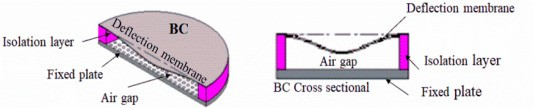
\includegraphics[width=1\linewidth]{img/MEMS_microphone_structure.jpg}
    \caption{MEMS microphone structure}
    \label{fig:MEMS_microphone_structure}
\end{figure}
\vspace{0.5cm}

\noindent
The goal is to detect pressure variations acting on the diaphragm. \\
To achieve this, two electrodes are connected to the structure in order to measure the variation in electrical capacitance between the diaphragm and the bottom plate. \\
The problem with the common structure shown above is that the air gap between the membrane and the bottom plate has a non-negligible viscosity, which can compromise the functionality of the microphone. \\
Air viscosity, in fact, modifies the ideal relationship that links pressure to the capacitance variation of the membrane. \\
The two structures considered are taken from the paper \cite{krishnapriya2014} and employ common strategies to reduce the effect of air viscosity in the gap. \\
The idea is to introduce holes either in the diaphragm or in the bottom plate to allow air to pass through them.

\section{Analyzed MEMS capacitive microphone structures}
The two microphone structures are fabricated on a silicon wafer on which an insulating layer has been grown. \\
On top of the insulating layer, the conductive backplate is deposited, and spacers to support the membrane are formed. \\
The lateral spacers must be non-conductive to prevent electrical shorting between the backplate and the diaphragm. \\
On top of the spacers, the membrane, made of aluminum, is placed.

\newpage
\noindent
The first structure has a perforated diaphragm and includes corrugations to facilitate membrane deflection in that region (\autoref{fig:perforated_diaphragm_cross_section}).

\begin{figure}[h!]
    \centering
    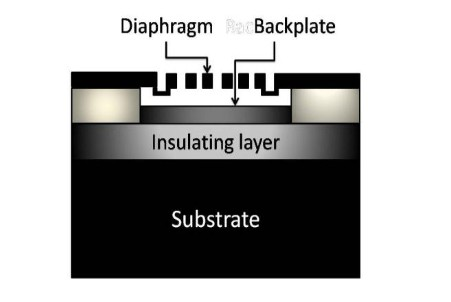
\includegraphics[width=0.7\linewidth]{img/perforated_diaphragm_cross_section.jpg}
    \caption{Cross section of capacitive microphone with corrugated and perforated diaphragm}
    \label{fig:perforated_diaphragm_cross_section}
\end{figure}

\noindent
The second structure has a corrugated membrane with no holes, but has a perforated backplate (\autoref{fig:perforated_backplate_cross_section}).

\begin{figure}[h!]
    \centering
    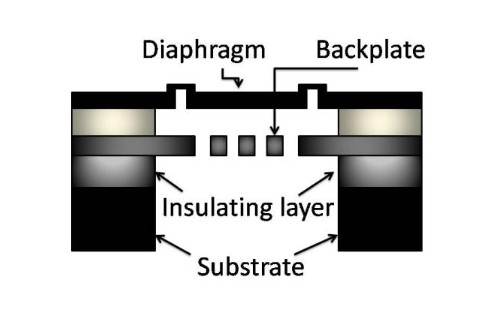
\includegraphics[width=0.7\linewidth]{img/perforated_backplate_cross_section.jpg}
    \caption{Cross section of capacitive microphone with perforated backplate}
    \label{fig:perforated_backplate_cross_section}
\end{figure}

\noindent
The main differences between these two structures are:

\begin{itemize}
    \item Air flows through the diaphragm holes in the first structure and through the backplate holes in the second structure.
    \item The perforated membrane is mechanically weaker than the solid one.
\end{itemize}

\noindent
As shown in \cite{jerman1986}, for shallow sinusoidal corrugations the deflection is approximately given by \cref{eq:diaphragm_deflection} \\

\begin{equation}
    \begin{cases}
        \frac{PR^4}{E'h^4} = a_p \frac{y}{h} + b_p \frac{y^3}{h^3} \\
        \\
        a_p = \frac{2(q+3)(q+1)}{3\left(1-\frac{v^2}{q^2}\right)} \\
        \\
        b_p = \frac{165(q+1)^3(q+3)}{q^2(q+4)(q+11)(2q+1)(3q+5)}
    \end{cases}
    \label{eq:diaphragm_deflection}
\end{equation}

\noindent
where:

\begin{itemize}
    \item \textbf{P}: Applied pressure
    \item \textbf{R}: Diaphragm radius
    \item \textbf{h}: Diaphragm thickness
    \item \textbf{y}: Diaphragm center deflection
    \item \textbf{v}: Poisson’s ratio
\end{itemize}

\noindent
The terms \(E^{'}\) and \(q\), for shallow sinusoidal profiles, are given by \cref{eq:E_param} and \cref{eq:q_param}:

\begin{equation}
    E^{'} = \frac{E}{1-v^2}
    \label{eq:E_param}
\end{equation}

\begin{equation}
    q = 1 + 1.5 \cdot \frac{H^2}{h^2}
    \label{eq:q_param}
\end{equation}

\noindent
where:

\begin{itemize}
    \item \textbf{E}: Young’s modulus
    \item \textbf{H}: Corrugation depth
\end{itemize}

\noindent
The approximated formula is more accurate for the perforated-backplate structure, because the membrane is corrugated without holes.


\section{Model Geometry in COMSOL}
The two models have been built in COMSOL Multiphysics. \\
The structures have been divided into five different domains (\autoref{fig:microphone_structure}):

\begin{itemize}
    \item \textbf{Diaphragm}: The membrane on which the pressure is applied
    \item \textbf{Backplate}: The bottom plate
    \item \textbf{Lateral borders}: The two insulating lateral spacers that separate the backplate from the diaphragm (every border is a separate domain)
    \item \textbf{Air gap}: The air region between the diaphragm and the backplate
\end{itemize}

\begin{figure}[h!]
    \centering
    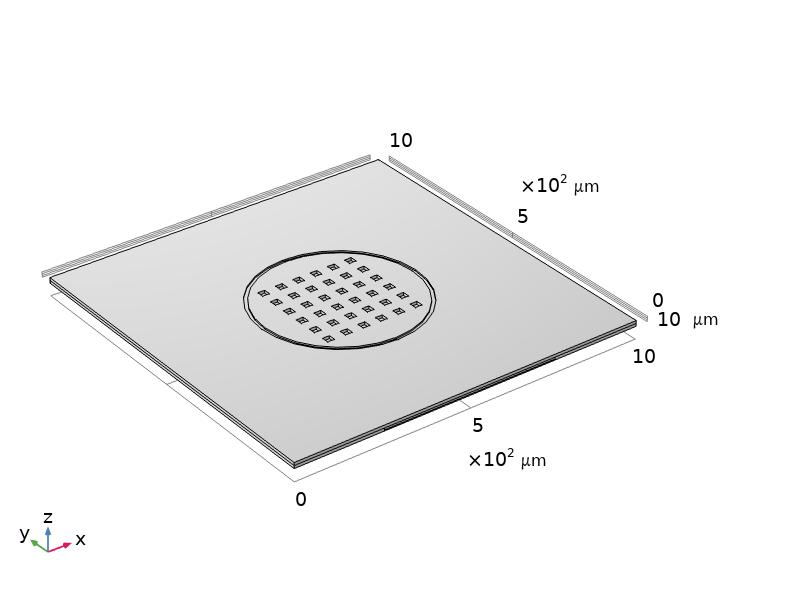
\includegraphics[width=0.95\linewidth]{img/microphone_structure.jpg}
    \caption{Microphone with perforated diaphragm model in COMSOL 6.4}
    \label{fig:microphone_structure}
\end{figure}

\newpage
\noindent
After defining the model structure and domains, the materials have been assigned:

\begin{itemize}
    \item The diaphragm and the bottom plate are made of aluminum
    \item The lateral borders are made of silicon dioxide ($SiO_2$)
    \item The gap between the diaphragm and the bottom plate is filled with air
\end{itemize}

\noindent
The final step in completing the model definition is to define the air gap as a moving mesh. \\
The top and lateral dimensions of the structure are shown in \autoref{fig:top_dimensions} and \autoref{fig:lateral_dimensions}, respectively.

\begin{figure}[h!]
    \centering
    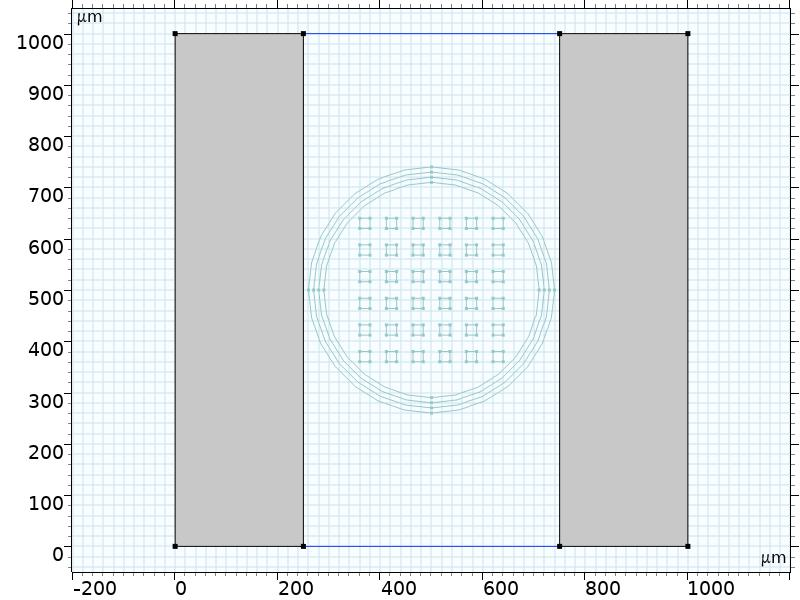
\includegraphics[width=0.95\linewidth]{img/top_dimensions.jpg}
    \caption{Top view of the MEMS microphone structure showing the main geometric dimensions in COMSOL 6.4.}
    \label{fig:top_dimensions}
\end{figure}

\begin{figure}[h!]
    \centering
    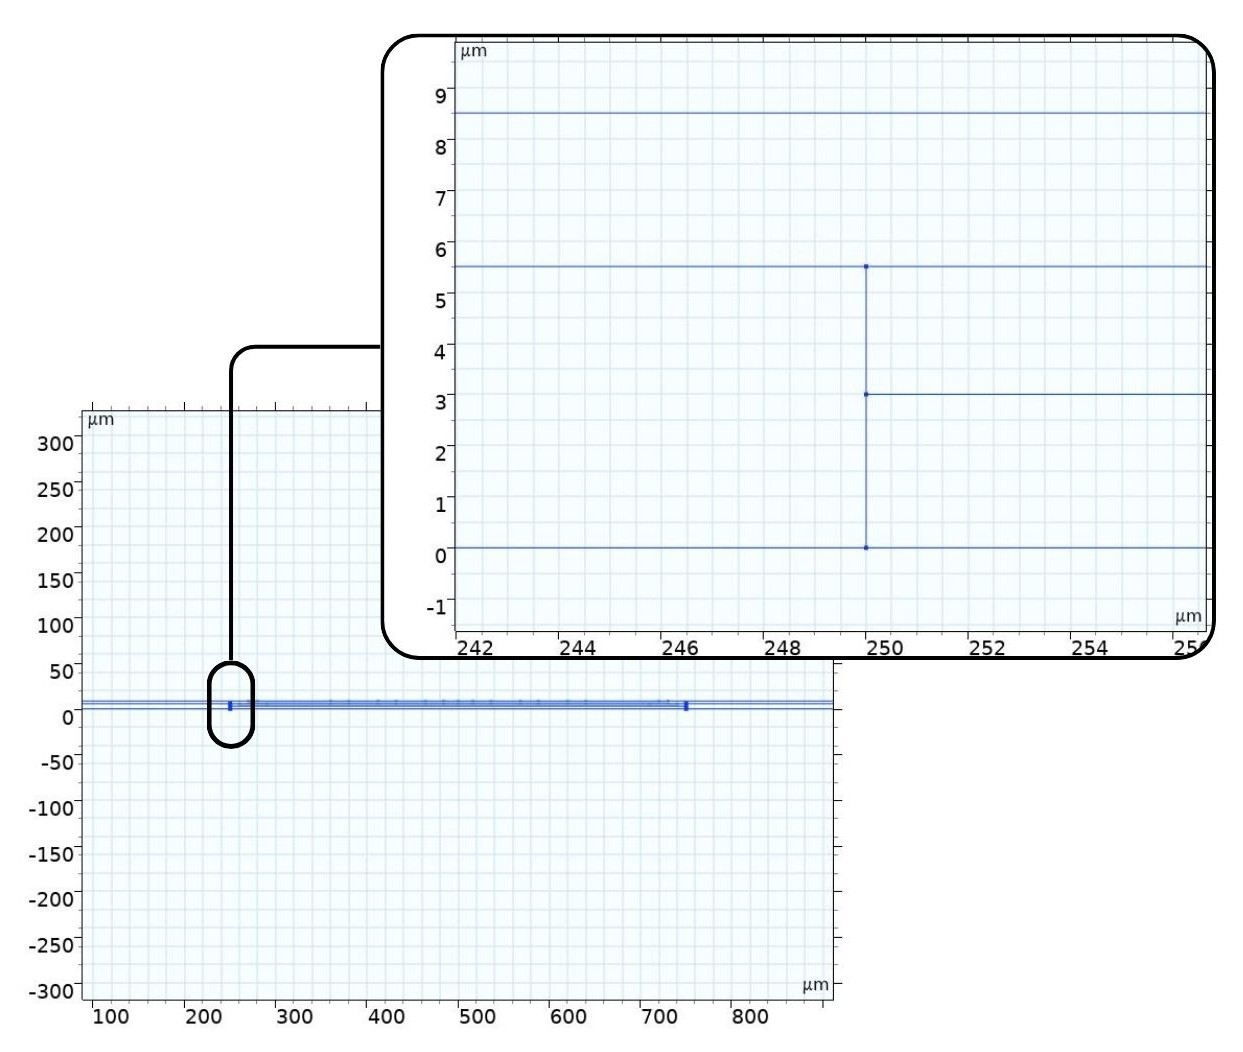
\includegraphics[width=0.95\linewidth]{img/lateral_dimensions.jpg}
    \caption{Lateral view of the MEMS microphone structure highlighting the vertical dimensions in COMSOL 6.4.}
    \label{fig:lateral_dimensions}
\end{figure}


\section{Definition of Physical Models in COMSOL}
The physics modules used are two:

\begin{itemize}
    \item \textbf{Solid Mechanics}: Module used to analyze the mechanical response of the structure to external loading
    \item \textbf{Electrostatics}: Module used to apply electrical charges and analyze the electric field in the structure
\end{itemize}

\noindent
The \textbf{Solid Mechanics} module is used to evaluate the membrane deformation and the resulting von Mises stress under applied pressure. \\
This deformation leads to a change in the capacitance between the membrane and the bottom plate, which can be measured to determine the pressure. \\
To compute this capacitance, a voltage is applied between the diaphragm and the bottom plate, and the \textbf{Electrostatics} module is used to simulate the voltage effect and calculate the capacitance.

\subsection[Solid Mechanics module parameters]{Solid Mechanics module \\ parameters}

All domains are defined as elastic materials, except for the air gap; this means that all domains operate in the elastic regime. \\
The module take the: Young's modulus (\(E\)), Poisson's ratio (\(v\)) and the density (\(\rho\)) from the materials. \\
All boundaries, except for the circular region inside the corrugation of the membrane (where the external pressure is applied, as shown in \autoref{fig:applyed_pressure}), are defined as free. \\
The bottom plate and the lateral border domains are defined with fixed constraints, while the circular region inside the corrugation of the membrane (\autoref{fig:applyed_pressure}) is set as a boundary load with an applied pressure.

\begin{figure}[h!]
    \centering
    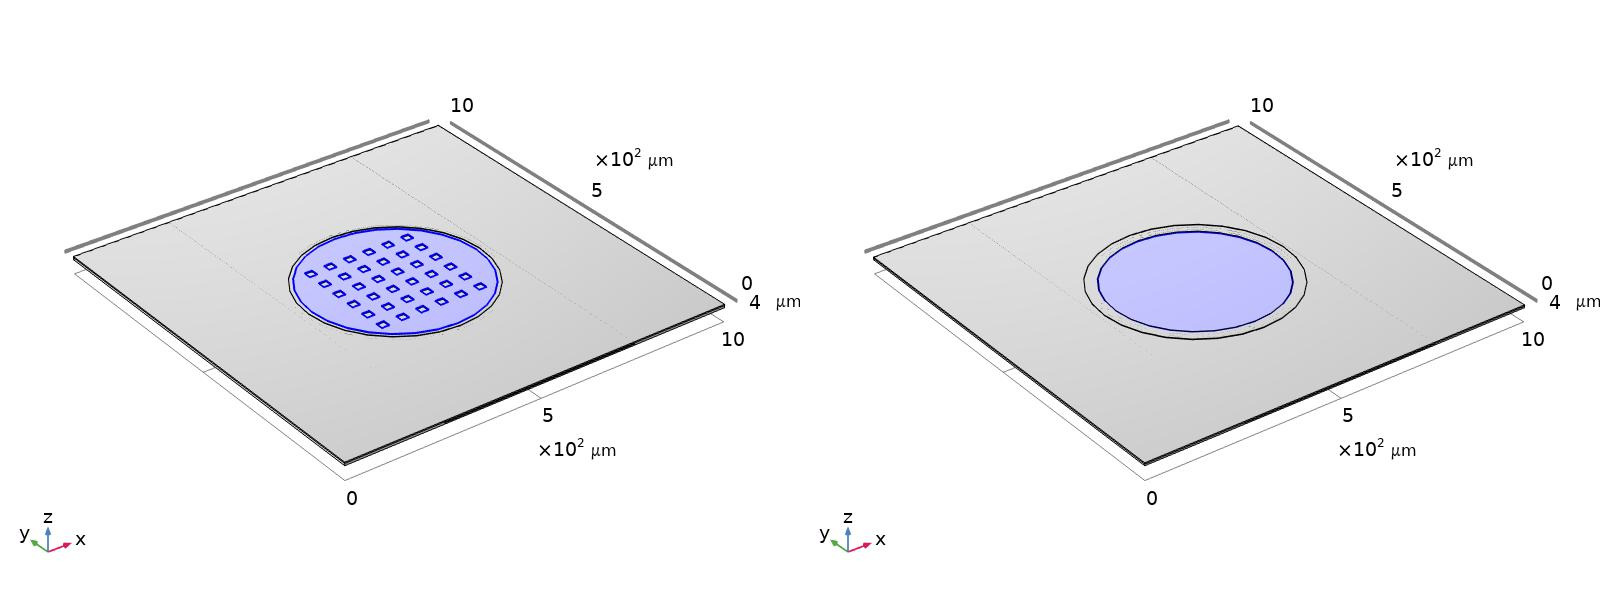
\includegraphics[width=1\linewidth]{img/applyed_pressure.jpg}
    \caption{In both structures, the region where the pressure is applied is highlighted: \\
    left is perforated diaphragm structure, right is perforated back structure}
    \label{fig:applyed_pressure}
\end{figure}

\newpage
\noindent
The initial conditions are the same for all domains, except for the air gap, and set both the initial displacement and the initial structural velocity to zero, as shown in \cref{eq:u=0} and \cref{eq:du/dt=0}.

\begin{equation}
    \vec{u} = (u_x, u_y, u_z) = (0, 0, 0) \; \mu m
    \label{eq:u=0}
\end{equation}

\begin{equation}
    \frac{\partial \vec{u}}{\partial t} = \frac{\partial}{\partial t}(u_x, u_y, u_z) = (0, 0, 0) \; \frac{\mu m}{s}
    \label{eq:du/dt=0}
\end{equation}

\subsection{Electrostatics module parameters}

The air gap domain is defined as free space; this means that, for this domain, the relation in \cref{eq:eps=0} holds.

\begin{equation}
    \epsilon_r = 1 \Rightarrow
    \vec{D} = \epsilon_0 \vec{E}
    \label{eq:eps=0}
\end{equation}

\noindent
All boundaries are defined as zero charge; this means that the charge density on those boundaries is zero, as shown in \cref{eq:rho=0}.

\begin{equation}
    \rho = 0 \; \frac{C}{m^2}
    \label{eq:rho=0}
\end{equation}

\noindent
The internal surface of the bottom plate is connected to ground (\(V = 0 \; V\)), and the diaphragm is defined as a terminal domain with an externally applied potential. \\
For the initial conditions, the potential of both the bottom plate and the diaphragm is set to zero.

\subsection{Multiphysics module parameters}

The \textbf{Multiphysics} module allows different physics interfaces to interact with each other. \\
The feature that enables the interaction between the \textbf{Electrostatics} and \textbf{Solid Mechanics} modules is the \textbf{Electromechanics, Solid} coupling. \\
The only domain selected for this coupling is the diaphragm domain.

\subsection{Mesh construction}

The mesh is automatically generated by COMSOL. \\
The mesh sequence is physics-controlled and defined as extra coarse due to the limited computational resources available on the computer used. \\
The structure is discretized into triangular and tetrahedral elements, and the number of generated entities for both structures is shown in \autoref{fig:mesh_perf_back} and \autoref{fig:mesh_perf_diap}.

\begin{figure}[h!]
    \centering
    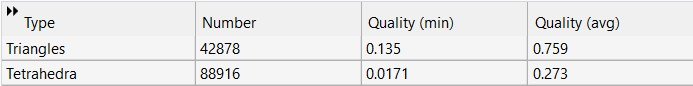
\includegraphics[width=1\linewidth]{img/mesh_perf_back.jpg}
    \caption{Number of mesh entities for the perforated backplate structure}
    \label{fig:mesh_perf_back}
\end{figure}

\begin{figure}[h!]
    \centering
    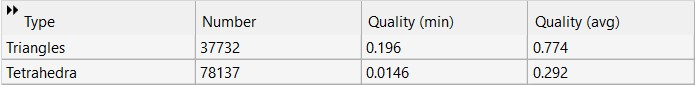
\includegraphics[width=1\linewidth]{img/mesh_perf_diap.jpg}
    \caption{Number of mesh entities for the perforated diaphragm structure}
    \label{fig:mesh_perf_diap}
\end{figure}

\begin{figure}[h!]
    \centering
    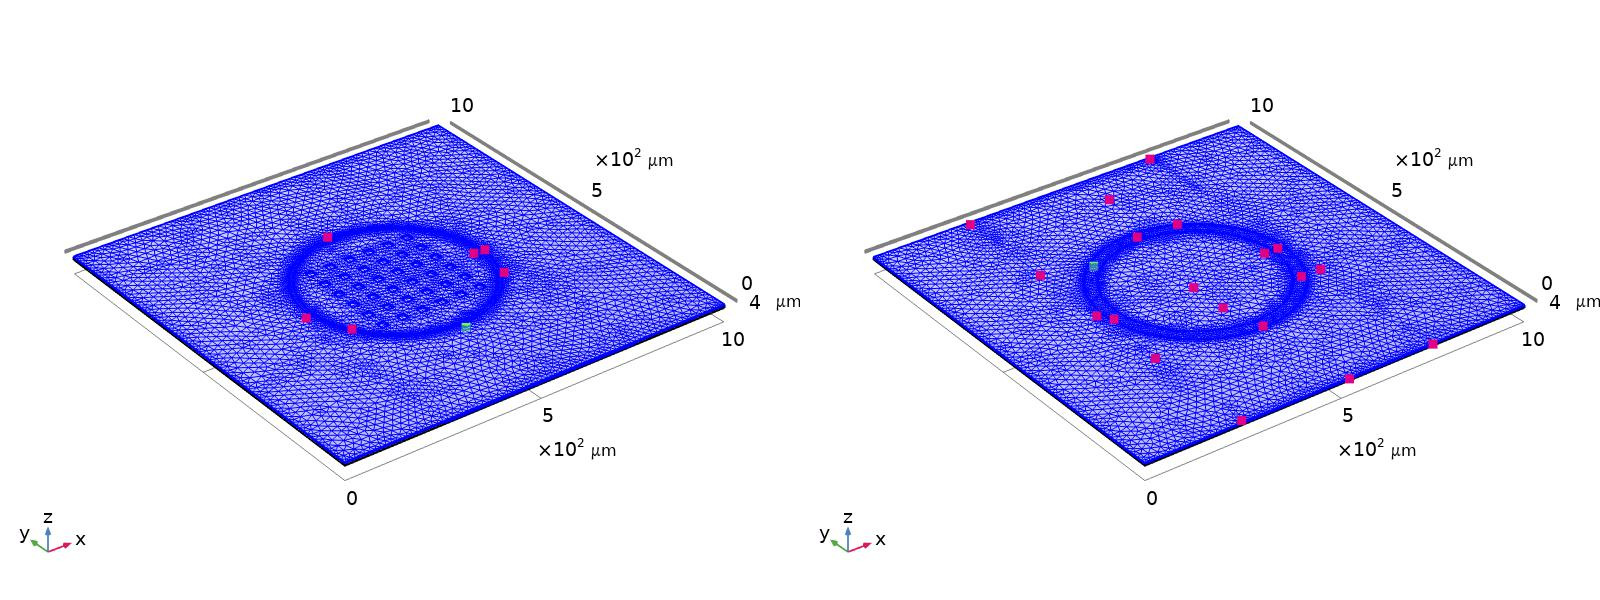
\includegraphics[width=1\linewidth]{img/mesh_build.jpg}
    \caption{Meshed structures: \\
    left is perforated diaphragm structure, right is perforated back structure}
    \label{fig:mesh_build}
\end{figure}

\section{Analysis of Simulation Results}
The simulation result will be compared with the result on the paper \cite{krishnapriya2014}. \\
The simulations were performed by varying two parameters:

\begin{itemize}
    \item \texttt{t\_d}: Membrane thickness
    \item \texttt{P\_x}: Applied external pressure
\end{itemize}

\noindent
The quantities of interest to be extracted from the results are:

\begin{itemize}
    \item \textbf{Displacement}: Membrane displacement
    \item \textbf{Stress}: Membrane von Mises stress
    \item \textbf{Sensitivity}: Maximum displacement per unit applied pressure
\end{itemize}

\subsection{Diaphragm Displacement}
The first quantity compared with the results reported in the reference paper is the membrane displacement. \\
The maximum displacement values for both structures differ from those reported in the paper. \\
This difference is expected, since the geometrical details of the holes and corrugations are not fully specified in the paper, leading to differences between the simulated and reference structures. \\
The most relevant observation is that, in the reference paper, the difference in maximum displacement between the two structures is significantly larger than in the simulations. \\
In fact, the maximum displacement reported in \cite{krishnapriya2014} ranges from \(0.7169 \; \mu m\) for the perforated diaphragm structure to \(0.4875 \; \mu m\) for the perforated backplate structure, whereas in the simulations the values range from \(0.585 \; \mu m\) to \(0.551 \; \mu m\), respectively, as shown in \autoref{fig:3d_displacement_module}.

\begin{figure}[h!]
    \centering
    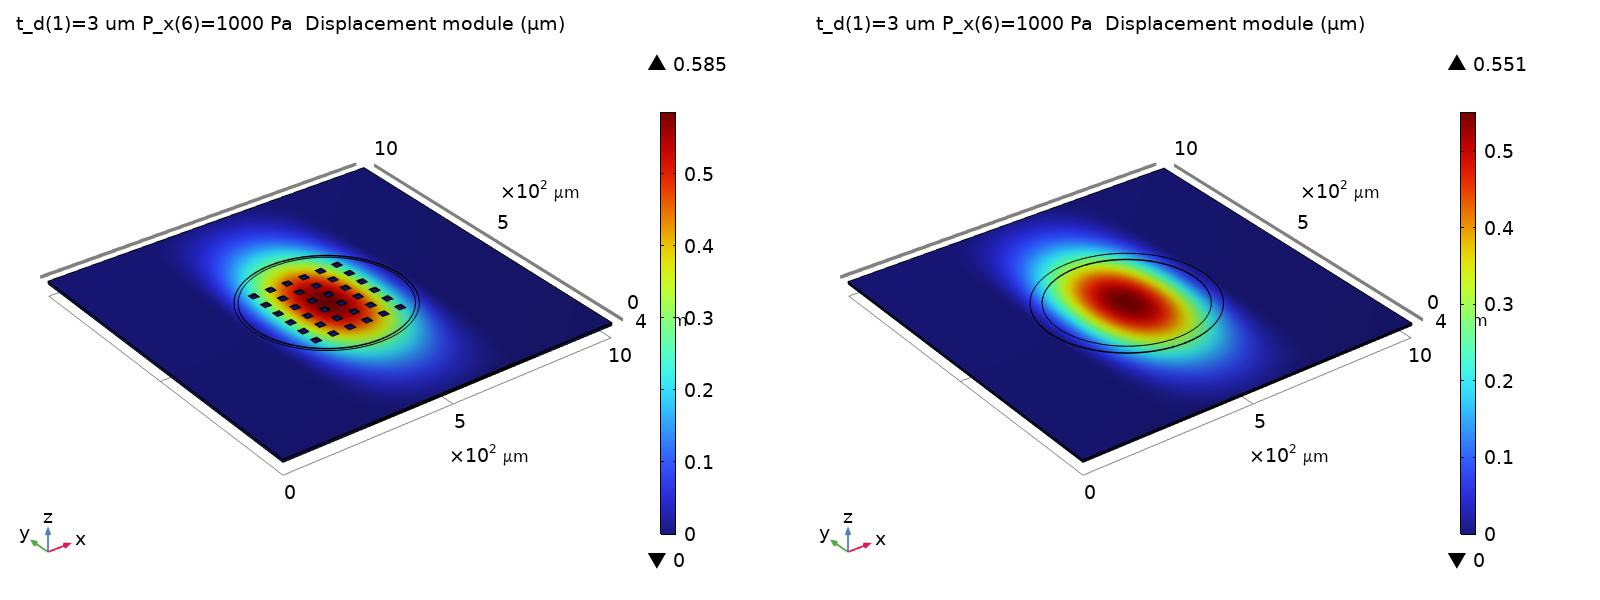
\includegraphics[width=1\linewidth]{img/3d_displacement_module.jpg}
    \caption{Displacement magnitude for both structures: \\
    left is perforated diaphragm structure, right is perforated back structure}
    \label{fig:3d_displacement_module}
\end{figure}

\noindent
It is important to specify that the displacement shown in \autoref{fig:3d_displacement_module} has been obtained with a diaphragm thickness (\texttt{t\_d}) of \(3 \; \mu m\), an air gap (\texttt{h\_air}) of \(1 \; \mu m\), and an applied external pressure (\texttt{P\_x}) of \(1000 \; \text{Pa}\), which are the same values used in the reference paper. \\
The difference in displacement values is due to the presence of holes in the membrane, which mechanically weaken the structure and result in a larger displacement under the same applied load. \\
Although the holes weaken the structure, the deformation trend as a function of position remains similar for both configurations. \\
To verify this, the displacement along a line on the diaphragm surface has also been evaluated.

\begin{figure}[h!]
    \centering
    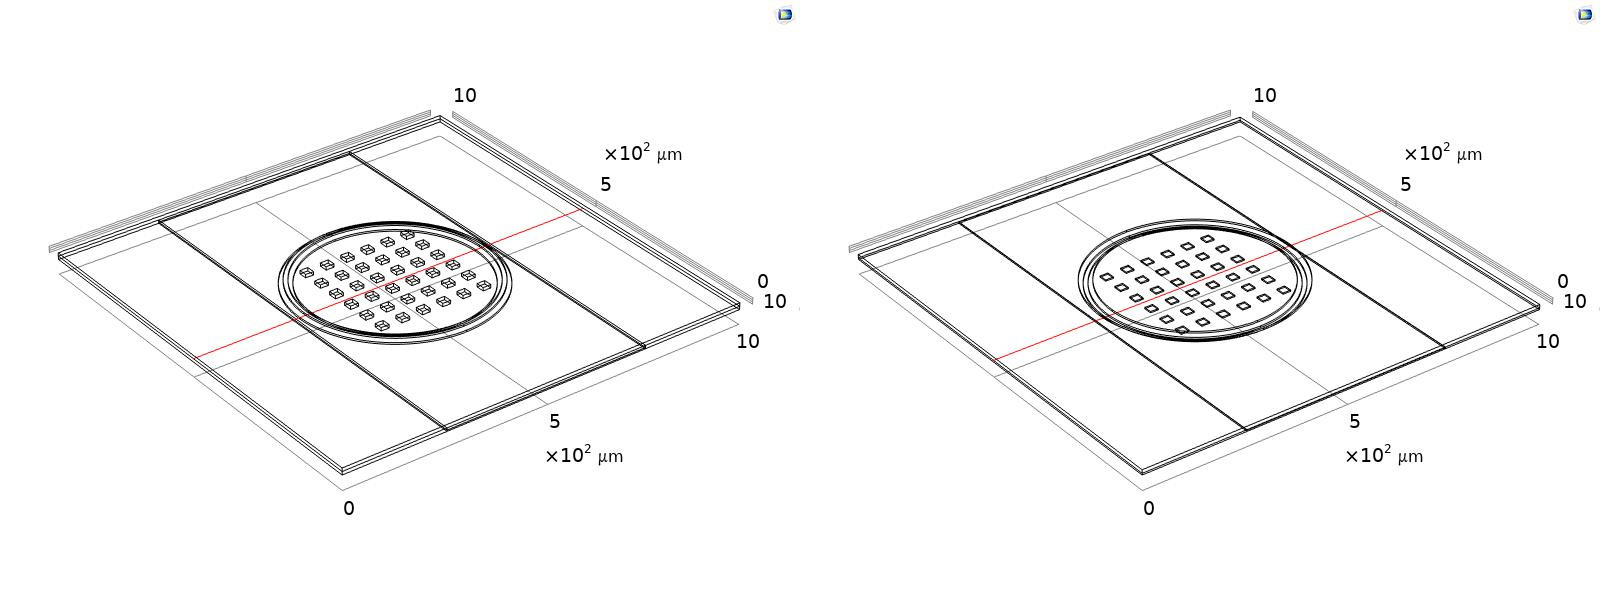
\includegraphics[width=1\linewidth]{img/center_line_visualization.jpg}
    \caption{Line along which the displacement is evaluated: \\
    left is perforated diaphragm structure, right is perforated back structure}
    \label{fig:center_line_visualization}
\end{figure}

\begin{figure}[h!]
    \centering
    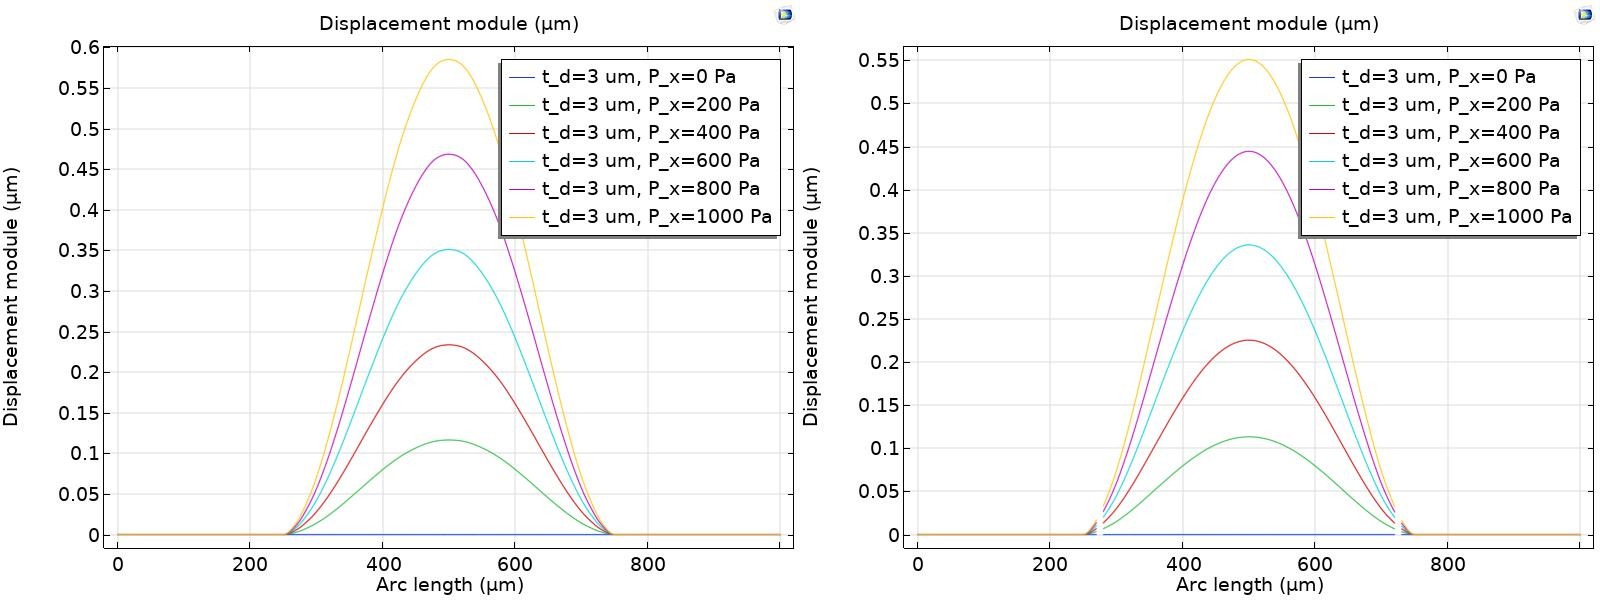
\includegraphics[width=1\linewidth]{img/center_line_displacement.jpg}
    \caption{Center-line displacement as a function of arc length, parameterized by applied pressure: \\
    left is perforated diaphragm structure, right is perforated back structure}
    \label{fig:center_line_displacement}
\end{figure}

\newpage
\noindent
As shown in \autoref{fig:center_line_displacement}, the displacement along the arc length follows the same trend for both structures; however, the perforated diaphragm structure always have a higher maximum displacement, as we expected. \\
It can also be observed that, by reducing the applied pressure, the difference in maximum displacement between the two structures becomes less significant. \\
Can be also interesting to analyze the behavior of the maximum displacement as a function of diaphragm thickness.

\begin{figure}[h!]
    \centering
    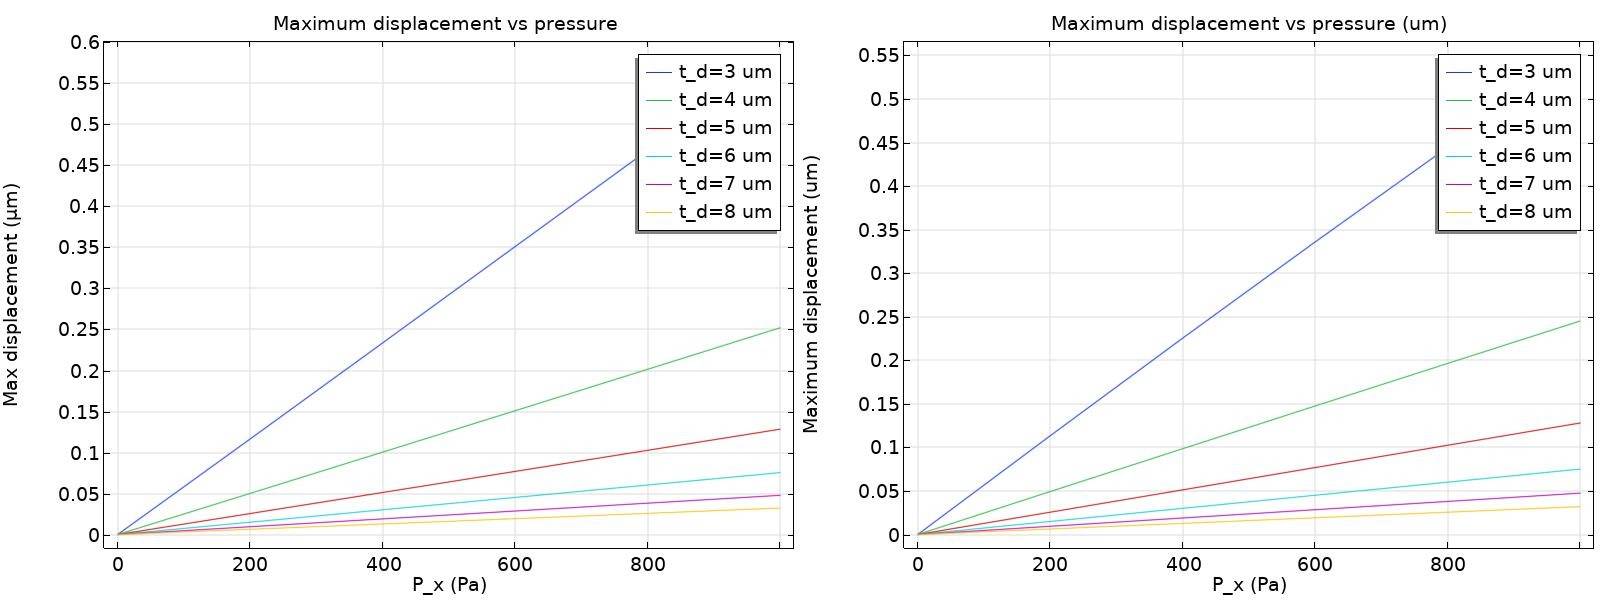
\includegraphics[width=1\linewidth]{img/maximum_disp_vs_pressure.jpg}
    \caption{Maximum center-line displacement as a function of applied pressure, parameterized by diaphragm thickness: \\
    left is perforated diaphragm structure, right is perforated back structure}
    \label{fig:maximum_disp_vs_pressure}
\end{figure}

\noindent
As shown in \autoref{fig:maximum_disp_vs_pressure}, the maximum displacement can be approximated as a linear function of pressure for the range of pressures and diaphragm thicknesses considered. \\
The displacement is always higher for the perforated diaphragm structure (concordant result with \cite{krishnapriya2014}); however, increasing the diaphragm thickness reduces the slope of the function, resulting in a smaller difference in displacement between the two structures. \\
Due to the linear trend of the function, reducing the applied pressure also leads to a decrease in displacement and, consequently, to a smaller difference in displacement between the two structures; this effect can also be observed in \autoref{fig:center_line_displacement}.

\subsection[Electromechanical Effects of Applied Bias Voltage]{Electromechanical Effects of \\ Applied Bias Voltage}

The voltage applied to the structure to measure the capacitance of the sensor generates an electric field in the air gap of the microphone, which attracts the membrane toward the bottom plate, causing a mechanical displacement of the diaphragm. \\
An interesting analysis consists in evaluating the membrane displacement induced only by the applied voltage (\autoref{fig:3D_voltage_displacement} and \autoref{fig:center_line_voltage_displacement}). \\
The simulation was performed without external pressure, with a diaphragm thickness (\texttt{t\_d}) of \(3 \; \mu m\), and with an applied voltage (\texttt{V\_x}) of \(1 \; V\). \\
As shown in \autoref{fig:3D_voltage_displacement}, the maximum displacement is \(7.68 \cdot 10^{-4} \; \mu m\) for the perforated diaphragm structure and \(1.09 \cdot 10^{-3} \; \mu m\) for the perforated backplate structure.

\begin{figure}[h!]
    \centering
    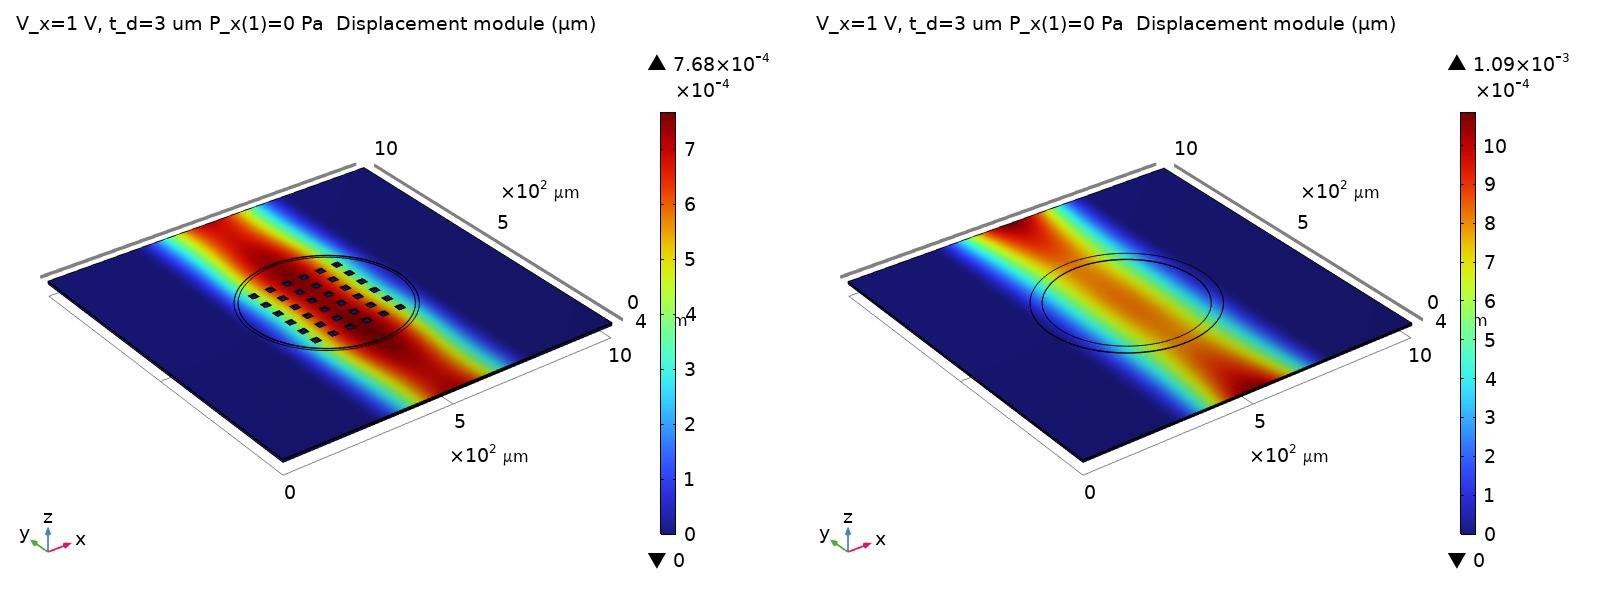
\includegraphics[width=1\linewidth]{img/3D_voltage_displacement.jpg}
    \caption{Displacement magnitude obtained without external pressure, induced only by the applied voltage: \\
    left is perforated diaphragm structure, right is perforated back structure}
    \label{fig:3D_voltage_displacement}
\end{figure}

\begin{figure}[h!]
    \centering
    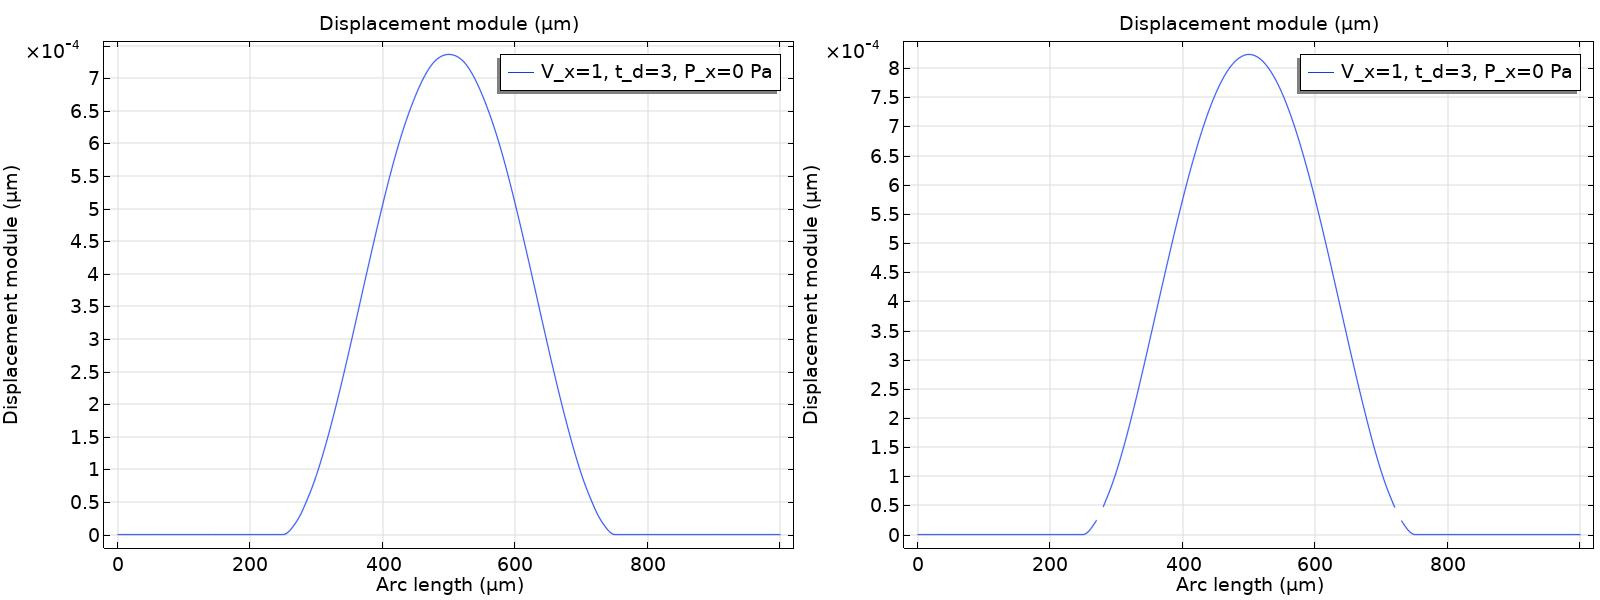
\includegraphics[width=1\linewidth]{img/center_line_voltage_displacement.jpg}
    \caption{Center-line displacement obtained without external pressure, induced only by the applied voltage: \\
    left is perforated diaphragm structure, right is perforated back structure}
    \label{fig:center_line_voltage_displacement}
\end{figure}

\noindent
These values do not match those shown in \autoref{fig:center_line_voltage_displacement} because the maximum displacement reported in \autoref{fig:3D_voltage_displacement} considers the entire membrane domain. In particular, the displacement at the membrane edges is greater than at its center. \\
For pressures greater than \(100 \; Pa\), the displacement values for both structures are more than two orders of magnitude larger; therefore, the displacement generated by the applied voltage is negligible in comparison. \\
Now, with bias voltage selected of \(1 \; V\) let's check the variation of Maxwell capacitance with pressure for both structures (\autoref{fig:Capacitance_vs_pressure})

\begin{figure}[h!]
    \centering
    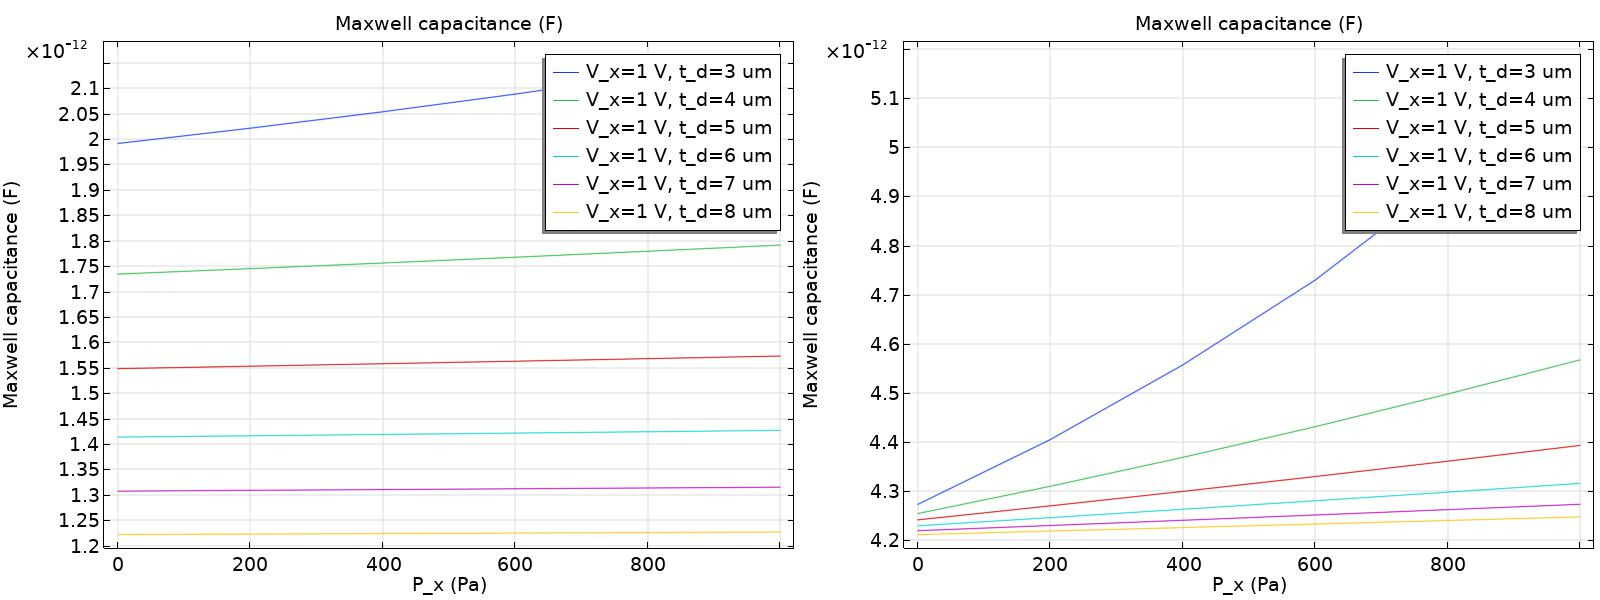
\includegraphics[width=1\linewidth]{img/Capacitance_vs_pressure.jpg}
    \caption{Capacitance vs external pressure applied: \\
    left is perforated diaphragm structure, right is perforated back structure}
    \label{fig:Capacitance_vs_pressure}
\end{figure}

\noindent
As shown in \autoref{fig:Capacitance_vs_pressure}, the capacitance is slightly higher for the perforated back structure, although the difference is not significant. \\
The most relevant aspect is the noticeable difference in capacitance sensitivity between the two configurations.

\begin{equation}
    \begin{aligned}
        \left. S_P^C \right|_{\text{perf. diap.}} & = \left. \frac{\partial C}{ \partial P} \right|_{\text{perf. diap.}} \\ 
        \frac{2.1663-1.991}{1000} \; \frac{pF}{Pa} & \simeq 0.1753 \cdot 10^{-3} \;\frac{pF}{Pa}
    \end{aligned}
    \label{eq:S_perf_diap}
\end{equation}

\begin{equation}
    \begin{aligned}
        \left. S_P^C \right|_{\text{perf. back}} & = \left. \frac{\partial C}{ \partial P} \right|_{\text{perf. back}} \\ 
        \frac{5.1897-4.2719}{1000} \; \frac{pF}{Pa} & \simeq 0.9178 \cdot 10^{-3} \; \frac{pF}{Pa}
    \end{aligned}
    \label{eq:S_perf_back}
\end{equation}

\noindent
The values in \cref{eq:S_perf_back} and \cref{eq:S_perf_diap} has been evaluated assuming a diaphragm thickness (\texttt{t\_d}) of \(3 \; \mu m\), a bias voltage (\texttt{V\_x}) of \(1 \; V\) and a linear approximation of the capacitance–pressure relationship.

\subsection{Diaphragm von Mises Stress}

The other quantity compared with the results reported
in the reference paper is the membrane stress.

\begin{figure}[h!]
    \centering
    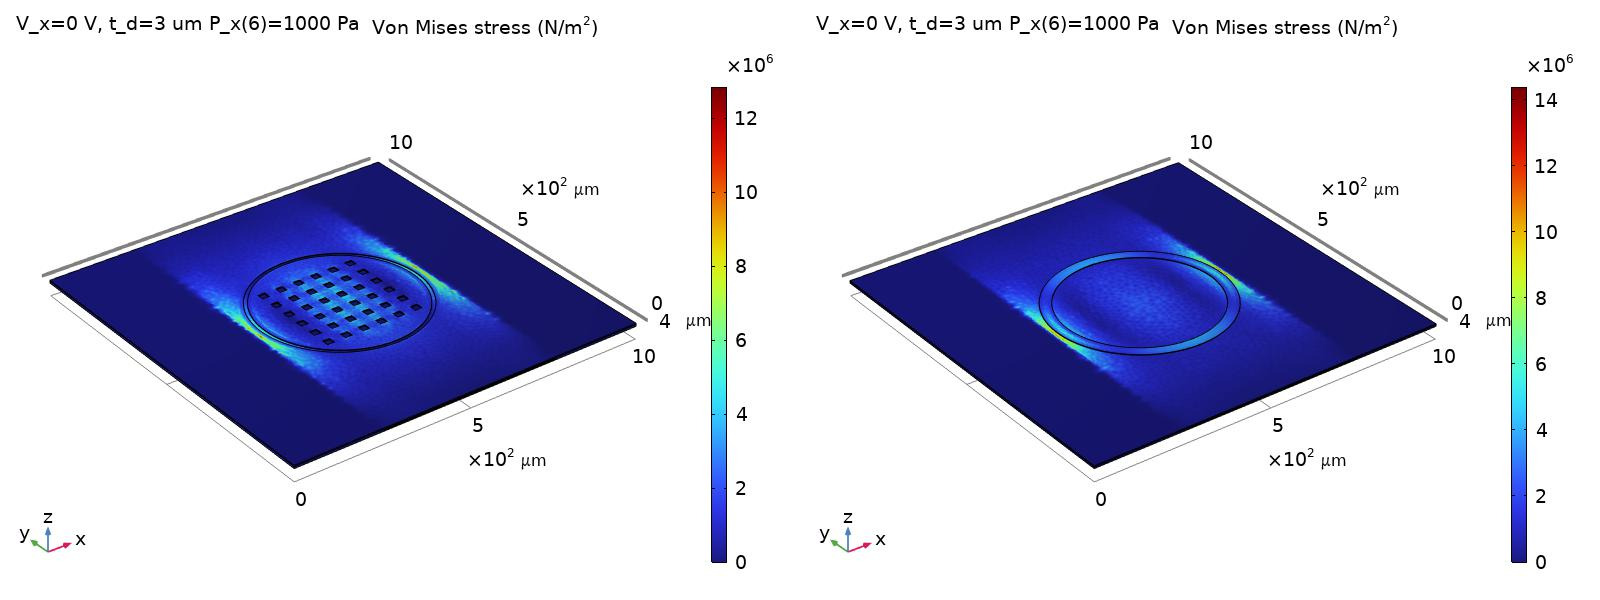
\includegraphics[width=1\linewidth]{img/3d_stress.jpg}
    \caption{von Mises stress for both structures: \\
    left is perforated diaphragm structure, right is perforated back structure}
    \label{fig:3d_stress}
\end{figure}

\noindent
As shown in \autoref{fig:3d_stress}, the maximum stress is located between the lateral edges and the corrugation of the membrane. \\
Within the corrugation, the stress is primarily concentrated at the center, while in the perforated diaphragm structure it increases near the edges of the holes. \\
The computed maximum stress is not fully representative, since the quantity of interest is the stress within the corrugation of the membrane. \\
However, the result is influenced by a stress peak at the membrane edge. \\
To better evaluate both the peak value and the stress distribution within the membrane, the stress profile along the center line has been analyzed. \\
The line along the stress has been evaluated is the same used for the displacement, shown in \autoref{fig:center_line_visualization}.

\begin{figure}[h!]
    \centering
    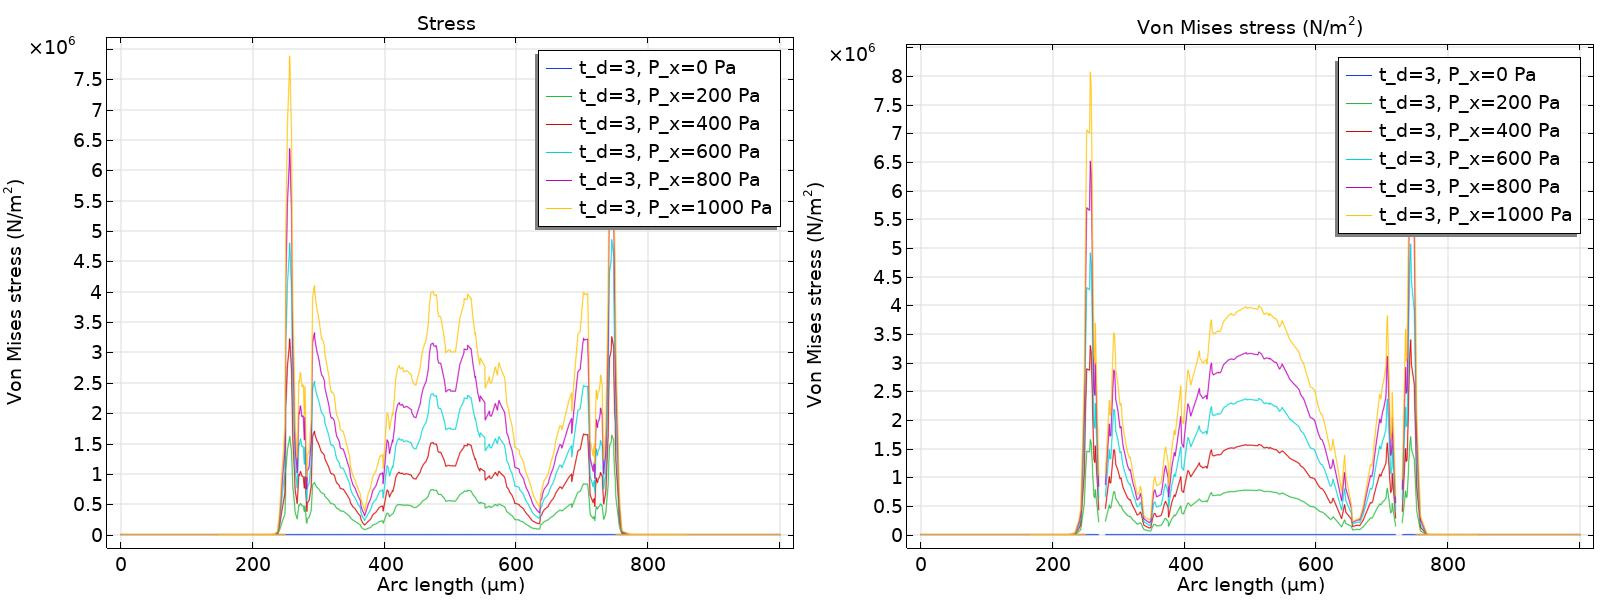
\includegraphics[width=1\linewidth]{img/center_line_von_mises_stress.jpg}
    \caption{Center-line von Mises stress as a function of arc length, parameterized by applied pressure: \\
    left is perforated diaphragm structure, right is perforated back structure}
    \label{fig:center_line_von_mises_stress}
\end{figure}

\newpage
\noindent
As we can see in \autoref{fig:center_line_von_mises_stress}, for the perforated diaphragm structure, the stress increases near the edges of the holes and decreases with increasing distance from them. \\
In contrast, for the perforated back structure, the stress distribution follows a trend that is closer to a quadratic profile. \\
Within the membrane region delimited by the corrugation, the maximum stress is nearly the same for both structures; the only difference lies in the stress distribution along the center line. \\
The stress also varies along the z-axis within the membrane (see \autoref{fig:MEMS_microphone_structure} for the axis orientation). The values shown in \autoref{fig:center_line_von_mises_stress} are evaluated along a line at the top surface of the membrane. \\
To obtain a more accurate estimate, excluding the stress peak near the lateral edges, the maximum stress at the top surface has been evaluated within the region delimited by the corrugation, that is also the area where the external pressure is applied (see \autoref{fig:applyed_pressure}).

\begin{figure}[h!]
    \centering
    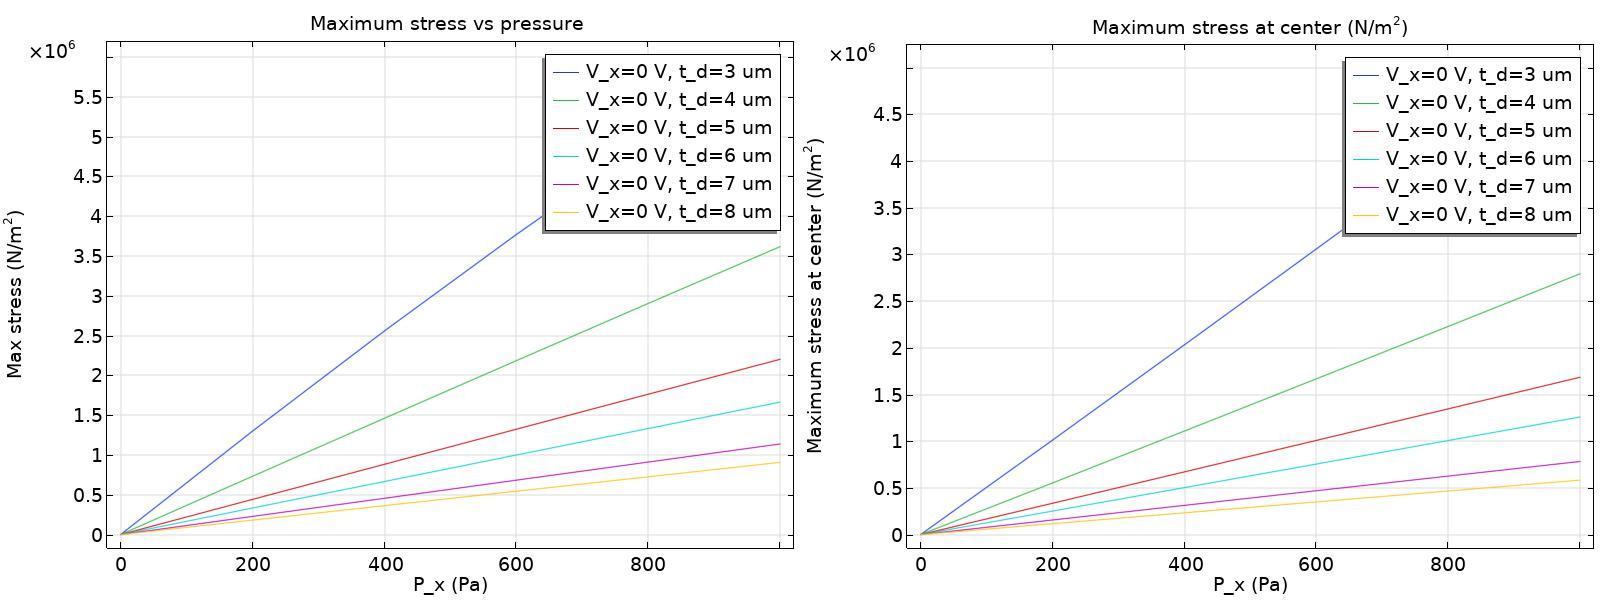
\includegraphics[width=1\linewidth]{img/maximum_stress_center_line.jpg}
    \caption{Maximum von Mises stress as a function of pressure applied, parametrized by diaphragm thickness: \\
    left is perforated diaphragm structure, right is perforated back structure}
    \label{fig:maximum_stress_center_line}
\end{figure}

\noindent
The stress, although less regular function than the displacement (along the center line), has a maximum value within the membrane that shows an approximately linear dependence on the applied pressure.

\newpage
\subsection[Displacement Sensitivity]{Diaphragm Displacement \\ Sensitivity}

The last parameter to be calculated is the displacement sensitivity of the membrane defined as \cref{eq:disp_sensitivity_definition}

\begin{equation}
    S_P^y = \frac{\text{maximum displacement}}{\text{pressure applied}} = \frac{max(|y|)}{P}
    \label{eq:disp_sensitivity_definition}
\end{equation}

\noindent
The perforated diaphragm structure has a weaker membrane; therefore, under the same applied pressure, it respond with a larger displacement. \\
For this reason, its displacement sensitivity is higher than that of the perforated back structure. \\
To verify this has been computed the displacement sensitivity as function of the applied pressure. \\
The maximum displacement value has been evaluated on the entire membrane domain for both structures (same method used to compute the maximum displacement on \autoref{fig:maximum_disp_vs_pressure})

\begin{figure}[h!]
    \centering
    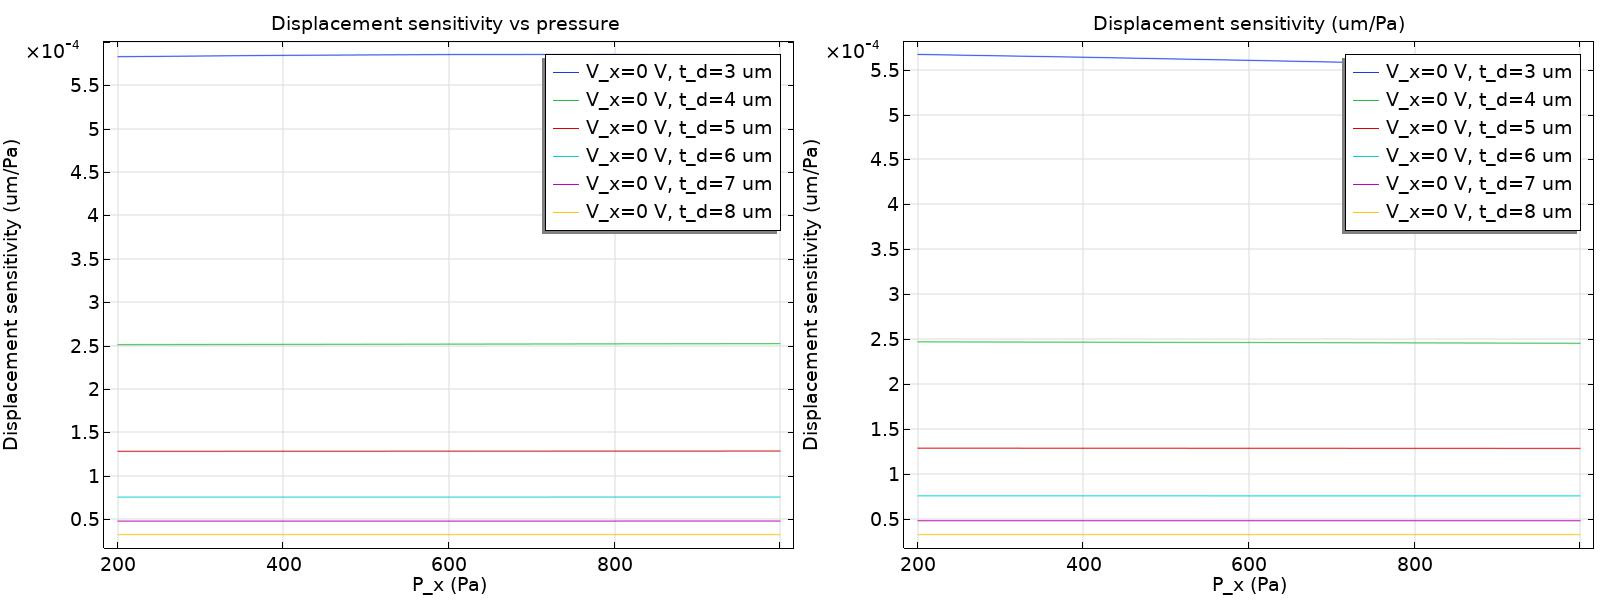
\includegraphics[width=1\linewidth]{img/displacement_sensitivity_parametrized.jpg}
    \caption{Maximum diaphragm displacement sensitivity as a function of pressure applied, parametrized by diaphragm thickness: \\
    left is perforated diaphragm structure, right is perforated back structure}
    \label{fig:displacement_sensitivity_parametrized}
\end{figure}

\noindent
As expected (\autoref{fig:displacement_sensitivity_parametrized}), the displacement sensitivity of the perforated diaphragm structure is higher than that of the perforated back structure. \\
However, due to the small difference in maximum displacement between the two configurations, the sensitivities are comparable. \\
The displacement sensitivity remains nearly constant with respect to pressure. \\
However, to better analyze its trend, the sensitivity was also evaluated with a single diaphragm thickness value.

\begin{figure}[h!]
    \centering
    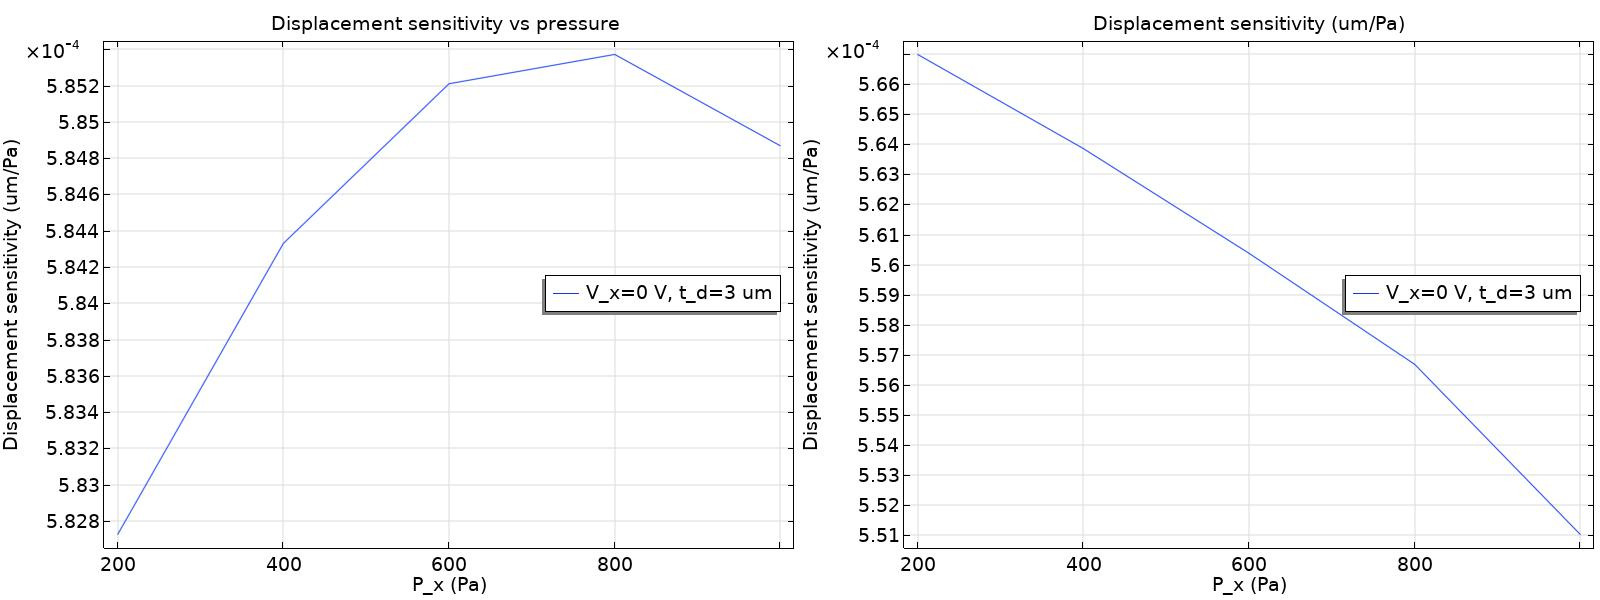
\includegraphics[width=1\linewidth]{img/displacement_sensitivit_trend_t_d=3um.jpg}
    \caption{Maximum diaphragm displacement sensitivity as a function of pressure applied, with a diaphragm thickness (\texttt{t\_d}) of \(3 \; \mu m\): \\
    left is perforated diaphragm structure, right is perforated back structure}
    \label{fig:displacement_sensitivit_trend_t_d=3um}
\end{figure}

\newpage
\noindent
From \autoref{fig:displacement_sensitivit_trend_t_d=3um}, graph obtained with a diaphragm thickness (\texttt{t\_d}) of \(3 \; \mu m\), we can see that for the perforated diaphragm structure the displacement sensitivity has an initially growing trend, which reaches a local maximum and then begins to decrease, and for the perforated back structure the trend is only decreasing. \\
To make a comparison, in the paper \cite{krishnapriya2014} the sensitivity is approximately constant with respect to the applied pressure, similarly to the simulation results. The reported values are \cref{eq:paper_sensitivity_value}

\begin{equation}
    \begin{aligned}
        \left. S_P^y \right|_{\text{perf. diap.}} &\simeq 7 \cdot 10^{-4} \; \mu\text{m}/\text{Pa} \\
        \left. S_P^y \right|_{\text{perf. back}} &\simeq 5 \cdot 10^{-4} \; \mu\text{m}/\text{Pa}
    \end{aligned}
    \label{eq:paper_sensitivity_value}
\end{equation}

The simulation results instead are \cref{eq:computed_sensitivity_value}

\begin{equation}
    \begin{aligned}
        \left. S_P^y \right|_{\text{perf. diap.}} &\in \left[5.82 ,\, 5.86\right]  \; \cdot 10^{-4} \mu\text{m}/\text{Pa} \\
        \left. S_P^y \right|_{\text{perf. back}} &\in \left[5.51 ,\, 5.67\right] \cdot 10^{-4} \; \mu\text{m}/\text{Pa}
    \end{aligned}
    \label{eq:computed_sensitivity_value}
\end{equation}

\noindent
As expected, the sensitivity values obtained from the simulations are of the same order of magnitude and show good agreement with the literature results for both structures.
This is because, as shown in \autoref{fig:3d_displacement_module}, the maximum displacement is almost the same in both cases; for this reason also the sensitivity values are similar. \\ 
The perforated back structure gives a maximum displacement that is close to the value reported in \cite{krishnapriya2014}. In contrast, the perforated diaphragm structure shows a larger difference. \\
For this reason, the results of the perforated back structure are closer to the reference paper values, while the other configuration differs more from them.

\newpage


\section{Conclusions}

In this report, two different types of microphone structures have been analyzed, and the results have been compared with each other and with the reference paper \cite{krishnapriya2014}. \\
The result are quite different from the paper for various reasons

\begin{itemize}
    \item The microphone structure in the paper is not fully defined, so the model used in this work has been built with slight modifications.
    \item The materials of the structure are defined in the paper, but the material properties used in the simulation may differ from those originally used.
    \item The physics modules used to perform the simulations are not specified in the paper.
    \item The mesh used is extremely coarse, this because of the computational cost of the simulation, leading to not accurate results.
\end{itemize}

\noindent
Another aspect to consider is that the structure has been analyzed without considering the air viscosity which introduces a nonlinear relationship between the displacement and the applied pressure. \\
Despite this, the computed results are physically plausible, considering the micromechanical properties of the structure. \\
An improvement to reduce the computational cost of the simulation is to exploit the symmetry of the structure; in fact, we can consider only a quarter of the structure and impose symmetry boundary conditions. \\
This approach could allow us to perform the simulations with a slightly improved mesh quality without increasing their computational cost.

\subsection{Comparison with paper results}

On the reference paper the displacement difference for both structures is larger than the one simulated, but comparing the displacement graph \cite[p.~3, Fig.~3 and Fig.~5]{krishnapriya2014}, with the one simulated (\autoref{fig:3d_displacement_module}) we can observe that the trend of the displacement on the structure is similar even if the values are different. \\
Another consideration that has to be done is that the perforated back structure shows results very close to those reported in the paper, both in terms of maximum displacement and displacement sensitivity. \\
The difference observed for the perforated diaphragm structure may be due to the inclusion of air viscosity effects in the original paper results.

\subsection{Mesh quality impact on results}

Surely the mesh quality introduced an error in the results, for this reason the two structures have been simplified, removing: the backplate, the air, the moving mesh, the parametric simulation and the electrostatic module, to allow the simulation with a better mesh quality and to see how the mesh impacts the final result.

\begin{figure}[h!]
    \centering
    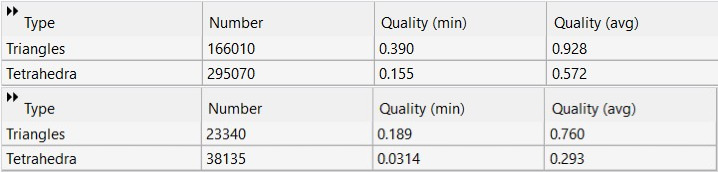
\includegraphics[width=1\linewidth]{img/perf_back_mesh_table.jpg}
    \caption{Number of mesh entities for the perforated back structure: \\
    the upper table is for normal quality mesh, the lower table is for extra-coarse quality mesh}
    \label{fig:perf_back_mesh_table}
\end{figure}

\begin{figure}[h!]
    \centering
    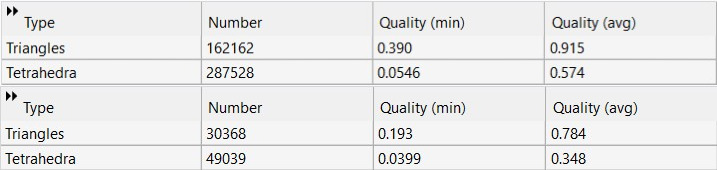
\includegraphics[width=1\linewidth]{img/perf_diap_mesh_table.jpg}
    \caption{Number of mesh entities for the perforated diaphragm structure: \\
    the upper table is for normal quality mesh, the lower table is for extra-coarse quality mesh}
    \label{fig:perf_diap_mesh_table}
\end{figure}

\noindent
The quantity evaluated with this two different type of mesh are the maximum displacement and the maximum stress values.

\begin{figure}[h!]
    \centering
    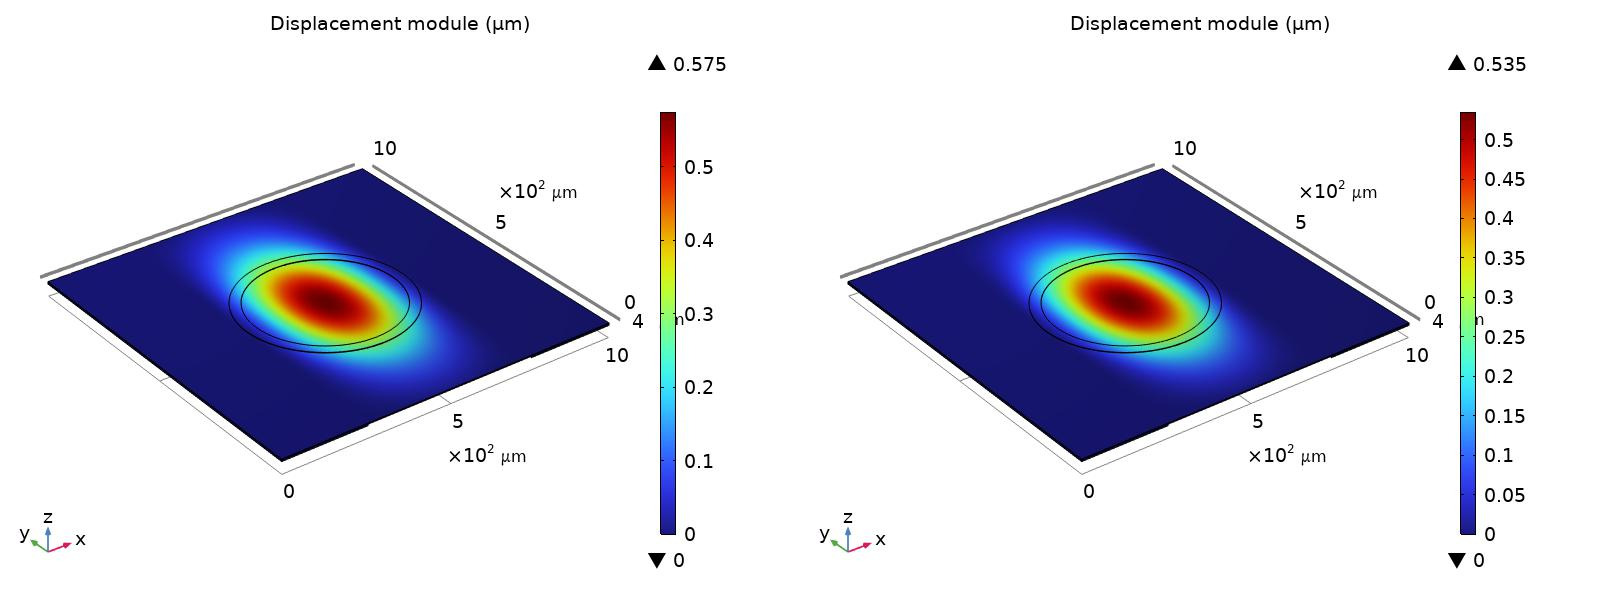
\includegraphics[width=1\linewidth]{img/displacement_mesh_impact_perf_back.jpg}
    \caption{Mesh impact on displacement for perforated back structure: \\
    left is normal quality mesh, right is extra-coarse quality mesh}
    \label{fig:displacement_mesh_impact_perf_back}
\end{figure}

\begin{figure}[h!]
    \centering
    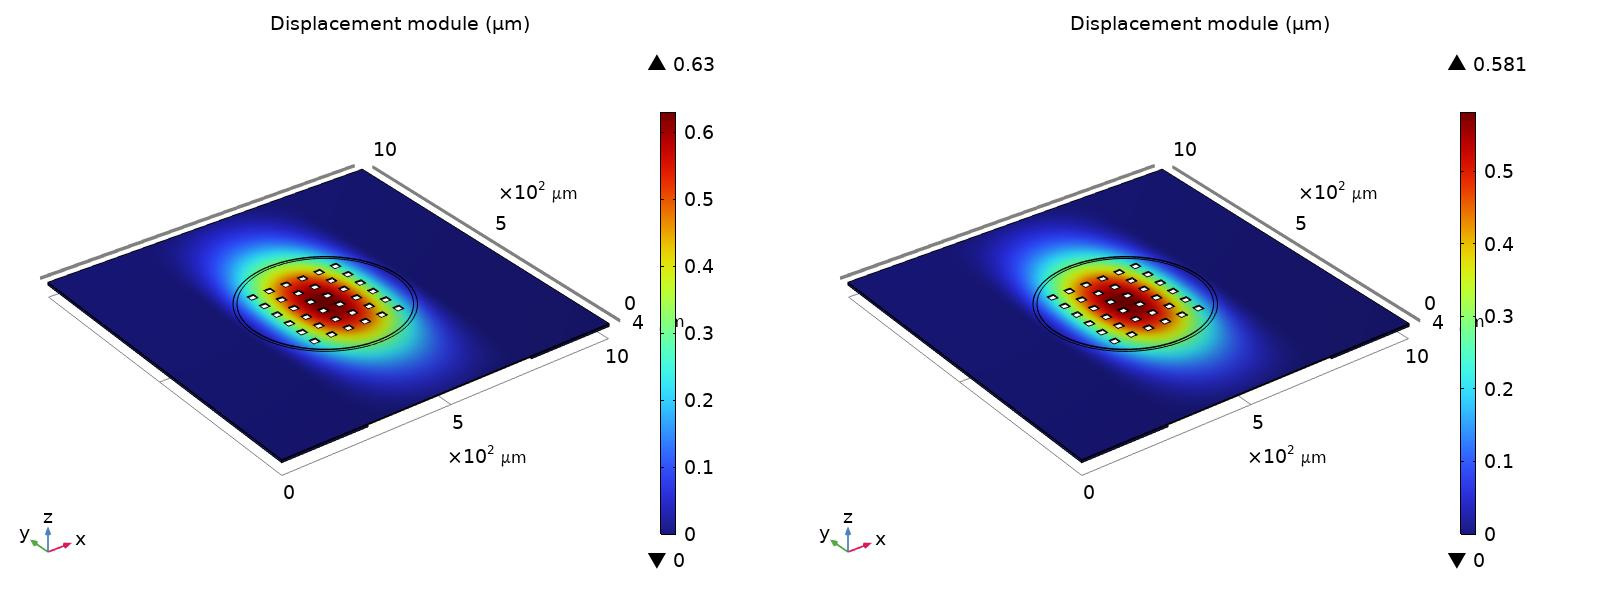
\includegraphics[width=1\linewidth]{img/displacement_mesh_impact_perf_diaph.jpg}
    \caption{Mesh impact on displacement for perforated diaphragm structure: \\
    left is normal quality mesh, right is extra-coarse quality mesh}
    \label{fig:displacement_mesh_impact_perf_diaph}
\end{figure}

\noindent
As we can see from \autoref{fig:displacement_mesh_impact_perf_back} and \autoref{fig:displacement_mesh_impact_perf_diaph}, the maximum displacement values decrease for both types of structure as the mesh quality decreases; this means that the larger displacement value shown is a more accurate approximation of the real value. \\
Obviously, these results are different from the ones obtained before, because the structures analyzed are simpler (to allow the computation with a higher-quality mesh). \\
These simulations has been done considering a diaphragm thickness (\texttt{t\_d}) of \(3 \; \mu m\), an applied voltage (\texttt{V\_x}) of \(0 \; V\) and an external pressure applied (\texttt{P\_x}) of \(1000 \; Pa\).
It can be interesting to evaluate the relative error induced by the mesh quality.
To calculate this, the formula \cref{eq:epsilon_r_formula} has been used.

\begin{equation}
    \varepsilon_r = \frac{ \left. f( \vec{r}) \right|_{\text{normal mesh}} - \left. f( \vec{r}) \right|_{\text{extra-coarse mesh}}}{\left. f( \vec{r}) \right|_{\text{normal mesh}}}
    \label{eq:epsilon_r_formula}
\end{equation}

\noindent
The absolute value of displacement relative errors are given by \cref{eq:epsilon_r_disp_perf_back} for the perforated back structure and by \cref{eq:epsilon_r_disp_perf_diap} for the perforated diaphragm structure.

\begin{equation}
    \left| \varepsilon_r \right|_{\text{perf. back}} \simeq \frac{0.575 \; \mu m - 0.535 \; \mu m}{0.575 \; \mu m} \simeq 0.0696
    \label{eq:epsilon_r_disp_perf_back}
\end{equation}

\begin{equation}
    \left| \varepsilon_r \right|_{\text{perf. diap.}} \simeq \frac{0.635 \; \mu m - 0.581 \; \mu m}{0.635 \; \mu m} \simeq 0.085
    \label{eq:epsilon_r_disp_perf_diap}
\end{equation}

\begin{figure}[h!]
    \centering
    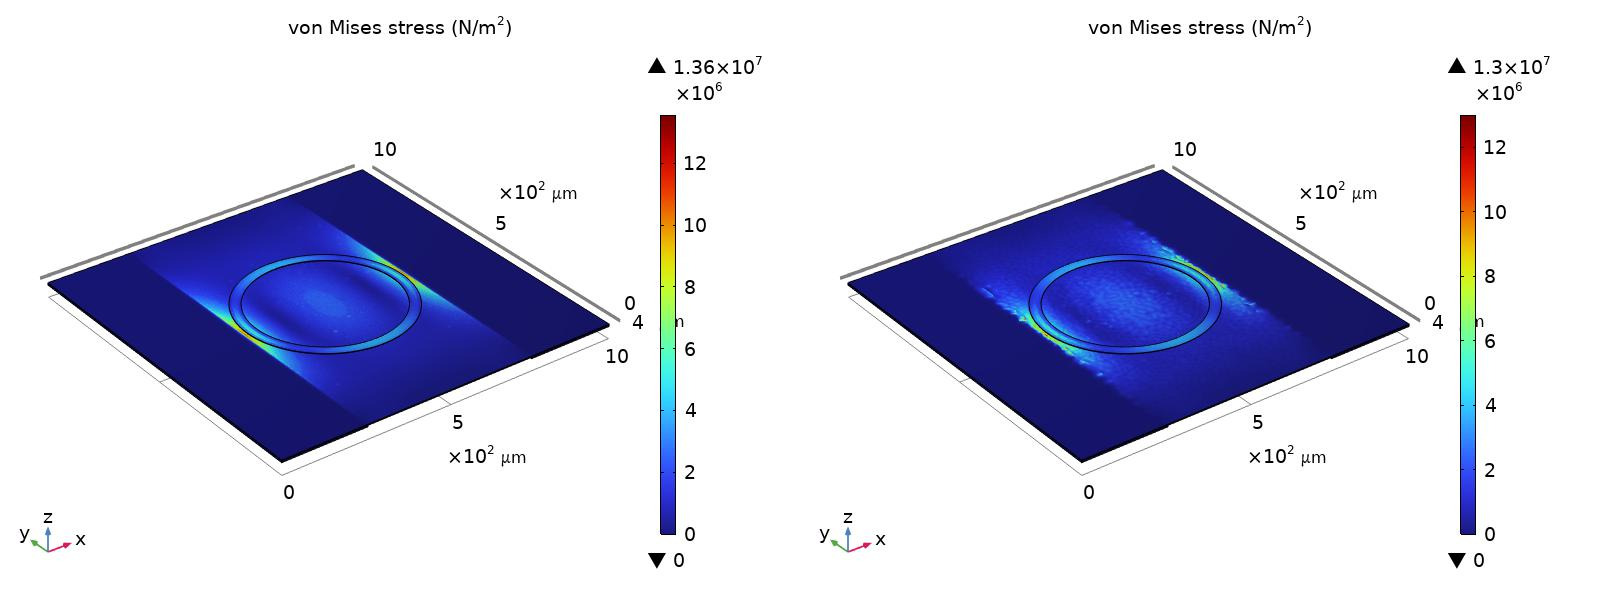
\includegraphics[width=1\linewidth]{img/stress_mesh_impact_perf_back.jpg}
    \caption{Mesh impact on von Mises stress for perforated back structure: \\
    left is normal quality mesh, right is extra-coarse quality mesh}
    \label{fig:stress_mesh_impact_perf_back}
\end{figure}

\begin{figure}[h!]
    \centering
    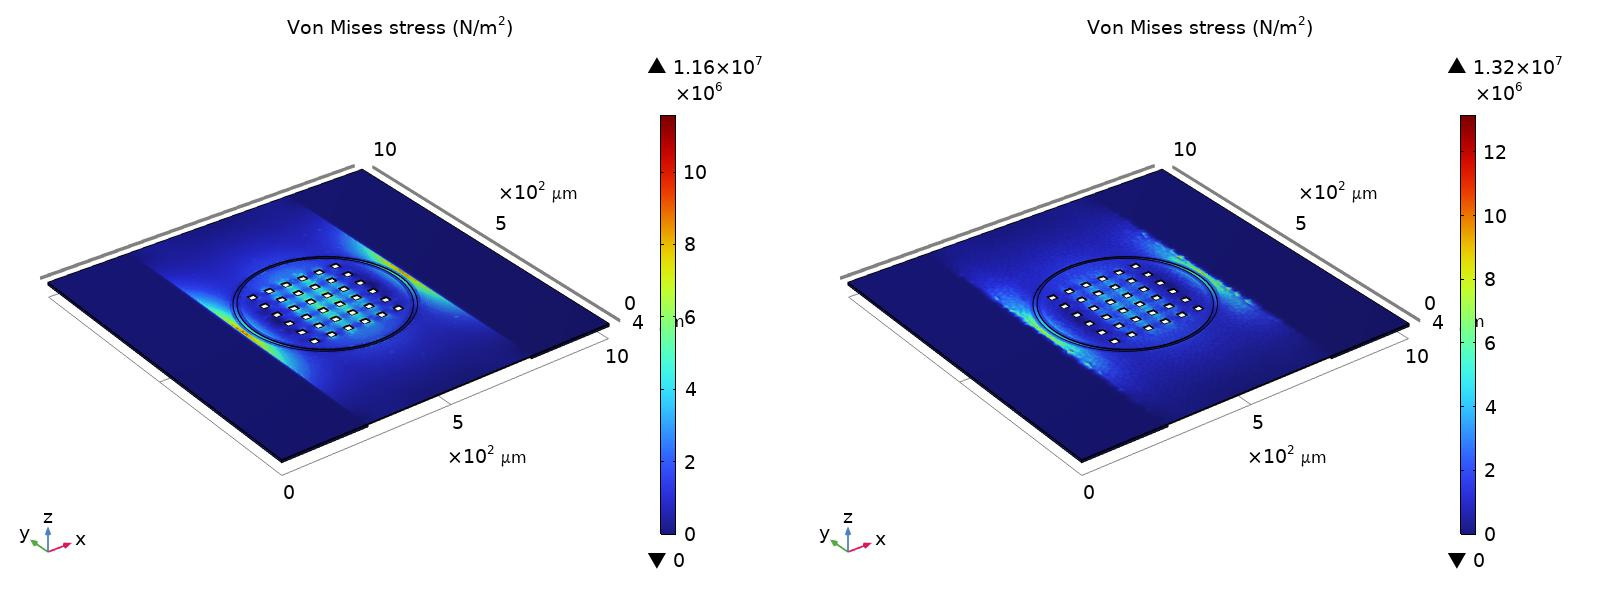
\includegraphics[width=1\linewidth]{img/stress_mesh_impact_perf_diaph.jpg}
    \caption{Mesh impact on von Mises stress for perforated diaphragm structure: \\
    left is normal quality mesh, right is extra-coarse quality mesh}
    \label{fig:stress_mesh_impact_perf_diaph}
\end{figure}

\noindent
The same evaluations has been done for the von Mises stress values as shown in \autoref{fig:stress_mesh_impact_perf_back} and \autoref{fig:stress_mesh_impact_perf_diaph}. \\
Differently from before, this time the evaluated maximum stress value does not decrease for both types of structure with the mesh quality. \\
This behavior can be caused by the peak value near the lateral border; probably, for a correct evaluation of that value, the mesh in that region must be very fine, otherwise the value is poorly approximated. \\
These simulations have been done with the same parameters as before, and by using the same formula to evaluate the absolute value of relative error (\cref{eq:epsilon_r_formula}), we can extract the errors for the stress values, which are respectively given by \cref{eq:epsilon_r_stress_perf_back} for the perforated back structure and \cref{eq:epsilon_r_stress_perf_diap} for the perforated diaphragm structure.

\begin{equation}
    \left| \varepsilon_r \right|_{\text{perf. back}} \simeq \frac{13.6 \; \frac{N}{mm^2} - 13 \; \frac{N}{mm^2}}{13.6 \; \frac{N}{mm^2}} \simeq 0.0441
    \label{eq:epsilon_r_stress_perf_back}
\end{equation}

\begin{equation}
    \left| \varepsilon_r \right|_{\text{perf. diap.}} \simeq \frac{13.2 \; \frac{N}{mm^2} - 11.6 \; \frac{N}{mm^2}}{11.6 \; \frac{N}{mm^2}} \simeq 0.138
    \label{eq:epsilon_r_stress_perf_diap}
\end{equation}

\noindent
As we can see from these results, the error goes from an approximately \(8.5 \%\) value for the displacement up to approximately \(13.8 \%\) for the stress values. \\
These error values are significant and may have caused the main difference from the results in the reference paper \cite{krishnapriya2014}.

\subsection{Comparison with analytical model and physical devices}

The last comparison done is the validity of the approximated analytical formula (found in the following paper \cite[p.~988-989]{jerman1986} for shallow, sinusoidal corrugated diaphragm) for the deflection of the membrane \cref{eq:diaphragm_deflection}. \\
To compute that, the following formula \cref{eq:plotted_disp_equation} has been plotted.

\begin{equation}
     \begin{cases}
        P = \frac{a_p}{\theta} \frac{y}{h} + \frac{b_p}{\theta} \frac{y^3}{h^3} \\
        \\
        \theta = \frac{R^4}{E'h^4}
    \end{cases}
    \label{eq:plotted_disp_equation}
\end{equation}

\noindent
The resulting graph has the pressure along the y-axis and the maximum displacement on the x-axis. \\
The displacement value associated with a specific pressure corresponds to the intersection of the graph with the function \(P=\texttt{P\_x}\), which corresponds to a horizontal line on the graph.
The data used for simulation, and to plot the graph are:

\begin{itemize}
    \item \textbf{h}: \(3 \; \mu m\) diaphragm thickness
    \item \textbf{H}: \(0,5 \cdot \text{h} = 1.5 \; \mu m\) corrugation depth
    \item \textbf{E}: \(70 \cdot 10^9 \; Pa\) Young's modulus for aluminum
    \item \textbf{v}: \(0.35\) Poisson's ratio for aluminum
    \item \textbf{R}: \(210 \; \mu m\) membrane ratio
\end{itemize}

\noindent
The resulting graph with the following values is shown in \autoref{fig:pressure_vs_disp}.

\begin{figure}[h!]
    \centering
    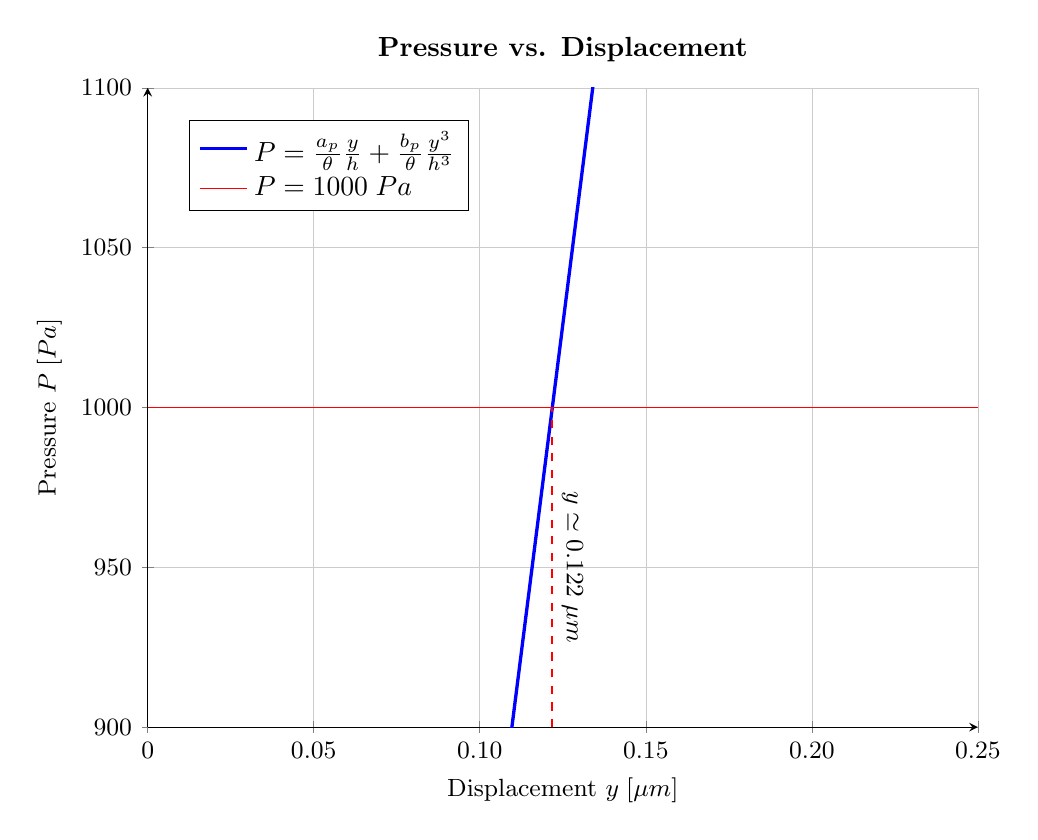
\begin{tikzpicture}
        \begin{axis}[
            width=\columnwidth,
            height=0.8\columnwidth,
            axis lines=left,
            xlabel={Displacement $y\;[\mu m]$},
            ylabel={Pressure $P\;[Pa]$},
            xmin=0, xmax=0.25,
            ymin=900, ymax=1100,
            grid=both,
            grid style={line width=.1pt, draw=gray!20},
            major grid style={line width=.2pt,draw=gray!40},
            legend style={at={(0.05,0.95)},anchor=north west},
            title={Pressure vs. Displacement},
            xtick = {0, 0.05, 0.1, 0.15, 0.2, 0.25},
            xticklabels = {$0$, $0.05$, $0.10$, $0.15$, $0.20$, $0.25$},
            ytick = {900, 950, 1000, 1050, 1100},
            yticklabels = {$900$, $950$, $1000$, $1050$, $1100$},
            title style={font=\bfseries},
            tick label style={font=\small},
            label style={font=\small},
            legend cell align={left}
        ]
        
        % Curve
        \addplot [blue, very thick, domain=0:0.25] {24609*x/3 + 7466*(x/3)^3};
        \addlegendentry{$P = \frac{a_p}{\theta} \frac{y}{h} + \frac{b_p}{\theta} \frac{y^3}{h^3}$}
        
        % Horizontal line
        \addplot [red, very thin] coordinates {(0,1000) (0.25,1000)};
        \addlegendentry{$P = 1000 \; Pa$}
    
        % Vertical line
        \addplot [red, dashed, thick] coordinates {(0.12184,900) (0.12184,1000)};
        \node[rotate=270, anchor=south, font=\small] at (axis cs:0.12184,950) {$y \simeq 0.122 \; \mu m$};
        
        \end{axis}

    \end{tikzpicture}

    \caption{Analytical pressure function plotted as a function of displacement}
    \label{fig:pressure_vs_disp}

\end{figure}

\noindent
As we can see from \autoref{fig:pressure_vs_disp}, the maximum displacement value at a pressure of \(1000 \; Pa\) is \(0.122 \; \mu m\), which is significantly different from the simulated results and from the values reported in the paper. \\
This confirms that the analytical function is only useful to get an idea of the order of magnitude we are working with.

\subsection{Final conclusions}

The simulations performed produced different results, and many parameters have been neglected. \\
The results vary significantly depending on several factors: mesh quality, model accuracy (simulating the entire device is different from simulating only the diaphragm), the analytical equations and the physical modules used for the simulations, etc. \\
For this reason, the mathematical approximated model and the simulations should only be used to size the structure, allowing us to understand the order of magnitude we are dealing with. \\
However, to design a proper MEMS microphone structure, many physical tests are required, because for complex structures like the one considered here, the results can differ significantly from the real ones. \\
Naturally, \textbf{COMSOL 6.4} is a powerful simulation tool that allows the coupling of different modules; the more physical modules are used, the more accurate the simulation results are, but the more complex the model becomes. \\
At a certain level of complexity, it becomes more convenient to perform simplified simulations and rely on physical tests.


\nocite{*}
\printbibliography

\end{document}